\chapter{Introduction}
\label{chp:introduction}

% What do I want to say and convey here?
% - scientific publications are the ``footprint'' and ``medium of discourse'' of academic progress
% - structured representation

% establish the nature and role of scientific publications
Scientific publications are the \emph{discourse medium} and \emph{literary footprint} of academic progress. As such, they play a vital role in the everyday workings and advancement of academia.
% segue to the digital
Historically, this role manifested itself physically---through ink on paper. In time, digital methods for authoring %/composition?
and distribution enabled more efficient ways of dissemination.
Today, scientific publications are predominantly authored, distributed, consumed, and archived digitally~\cite{Lamers2018}. However, the form of today's digital publications still retains numerous and deep traces of its physical ancestry.

% Digital dissemination makes the transfer of new knowledge into the research community faster and cheaper. Digital archives enable search technology and analytics to operate on our \emph{literary footprint} of past and present academic progress. In this way, digitization facilitates both faster progress in science, \emph{and} technology helping scientists to keep up with the increase in speed. However, today's form of digital publications is far from optimal for powering such technology. In fact, the form of today's digital publications poses significant challenges for 

% While there lies enormous potential in a digital record of science, there remain significant challenges to realizing this potential. A key cause of these challenges is the historical baggage of today's digital publications. This dissertation is in pursuit of tackling these challenges.

% There lies enormous potential in a digital record of science. But realizing this potential

The historical baggage manifesting itself in the PDF files we read, share, and author, poses significant challenges to realizing the full potential of a digital record of science. While digital services in academia such as search and recommendation do exist, they are powered not by publications themselves, but rather by more structured, derivative representations of publications. The same holds for analyses of publications (see Figure~\ref{fig:introduction-structreps}). Creating such structured representations %/derivates?
is challenging and error-prone, leading to a risk of subpar services and erroneous analyses. This dissertation represents an effort to tackle this challenge and alleviate the quality of structured representations of scientific publications.

% (random alliteration: structured surrogates of academic archives)

% - b/c of discrepancy between current form and what would be even better for digital dissemination and use (e.g. more structured), structured derivates of publications that enable digital services are of limited quality
% - historical baggage in part b/c still meant for human consumption
% - gap(?) between “pure” digital form and current form hinders more efficient use in digital services surrounding publications and academia

\begin{figure}[h]
  \centering
  
\includegraphics[width=\linewidth]{figures/introduction/structured_representations_of_publucations}
  \caption[Visualisation of publications, their structured representations, and their use]{Visualisation of publications, their structured representations, and their use.}
  \label{fig:introduction-structreps}
\end{figure}

\section{Scope and Motivation}

% What do I want to say and convey here?
% - why do we have/need scholarly data?
% - in contrast to intro paragraphs above, make *necessity* of scholarly data for mitigating information overload clear
% - also make clear why there was realistic potential in approaching the challenge

% Scholarly documents: research papers, project proposals, technical reports and academic documents
% 

% We first lay our the scope of the subject we consider as well as its significance. Based on this, we derive the motivation of the research project.

The focus subject of this dissertation are \textit{structured representations of scientific publications}%
%. For the sake of brevity, we will use the term ``scholarly data'' synonymously %
%\footnote{Note that in other contexts the term ``scholarly data'' can have a broader meaning than just ``structured representations of scientific publications''. For example, it can also include data on research institutions or funding bodies, without necessitating the context of a publication.} 
% and define the concept as follows.
, which we define as follows.

\begin{quote}
\textbf{Structured Representations of Scientific Publications}: Data representing the properties and contents of pieces of scientific literature in a structured way.
\end{quote}

For the sake of brevity, we use the term ``scholarly data'' synonymously.

\begin{quote}
\textbf{Scholarly Data}: Term used synonymously to ``structured representations of scientific publications'' in the context of this dissertation.
\end{quote}

% In other contexts, above terms can have a broader meaning and include, for example, data on research institutions or funding bodies, without necessitating the context of a publication.
% In the broadest sense, a collection of PDF files ... (NOTE: Scholarly data ``defined'' again in ch 2.1)
% Scholarly data, as defined above rooted in
% Being based on scientific literature, scholarly data is both a product
%\footnote{Note that in other contexts the term ``scholarly data'' can have a broader meaning than just ``structured representations of scientific publications''. For example, it can also include data on research institutions or funding bodies, without necessitating the context of a publication.} 

The importance of scholarly data, specifically large-scale scholarly data that is of high quality, lies in its potential as a remedy to challenges brought by the digitization of academic publishing.

% * in the olden days there were polymaths
% * nowadays an expert can't humanly keep up with their field
% * → we need assistance
% * → my research in on enabling the creating of such assistance

% * since ever, humans have sought shortcuts
% * in decision making in science: h-index etc. (not sure if this fits b/c I don't specifically address such metrics)

The digitization of academic publishing has made the transfer of new knowledge into the research community faster, thereby enabling an acceleration of scientific progress. A second driver of acceleration is the increase in research spending across the world~\cite{CRS2022,OECD2023}.
This increase in scientific progress, while first and foremost a positive development, brings with it a growing challenge for researchers to keep up with the literature. This problem is referred to as ``information overload''~\cite{Landhuis2016}.
Fortunately, the digitization of academic publishing not only lead to %/facilitated
an increase in the rate at which research results are being published. It also marks the inception of scholarly data, and thereby enabled search technology and analytics to operate on large collections of digitally archived publications.
In this way, the existence of digital representations of publications also provides, to some degree, a remedy for information overload. Efficient search and recommendation services, for example, can aid researchers in navigating the deluge of publications they are faced with.
Similarly, decision processes in academia, such as the evaluation of institutions or researchers, is enabled by scholarly data through performance indicators. In this way, it provides a means for hiring and funding decisions.
In other words, scholarly data is a vital resource for decision making in academia on the individual as well as organisational level.

The quality of decisions made based on scholarly data, naturally, hinges on the quality of the scholarly data itself. If, for example, citations are missing in the data of a search engine, this can cause researchers to overlook relevant related work, or a funding body to under-evaluate an institution. Recalling that the creation of scholarly data is a challenging and error-prone process, it stands to reason that efforts to improve scholarly data quality are a worthwhile endeavor. Based on these considerations, the overarching objective pursued in this dissertation is the development of methods for creating high-quality scholarly data.

% * not only is my research addressing the now pressing and increasing issue of an increasing rate of publication
% * it also tackles blind spots the have been left unaddressed for long (x-ling)

\section{Research Objective}\label{sec:intro-researchobj}

% What do I want to say and convey here?
% - make approached problem more concrete
%   - hand-wave-y in above:
%       ``[digital services in academia] are powered not by publications themselves,
%         but rather by more structured, derivative representations of publications''
%     -> publications authored by humans for humans -> scholarly data secondary/derivate
%     => concretization: derive structured representation from publications
%   - ``high-quality''
%     -> briefly touch upon what's laid out in foundation chapter
%     => concretization: high quality = fitness for use
% - (maybe even narrow down to reference focus, maybe *even* more to LaTeX based)
% - give example

To define our research objective, we need to take a closer look at what ``creating high-quality scholarly data'' entails. As briefly laid out above, scholarly data is a derivative product of publications. This is due to the fact that, for the time being, scientific publications are written by humans for humans. Because the product of this process---i.e., scientific literature in the form humans consume it in---is not well suited for digital processing \emph{as is}, scholarly data is created as a derivate based on publications. To make this creation process feasible on a large scale, it has to be automated.

Accordingly, we can define our research objective as follows.

\begin{infobox-objective}
\textbf{Research Objective}\\
Develop an automated process that takes as input scientific publications, and produces as output a high-quality derivative representation of the publications, suitable for digital processing.
\end{infobox-objective}

This leaves the question of what ``high-quality'' and ``suitable for digital processing'' entail. We discuss this aspect in detail in Chapter~\ref{chp:foundations}. In short, data quality depends on the intended use and therefore, generally speaking, means \emph{fitness for use}. Quantitatively, data quality is most commonly assessed along the following five dimensions~\cite{Herzog2007}.

\begin{infobox-progress}
      \textbf{Data Quality Dimensions}\\
       (1)~relevance, (2)~accuracy, (3)~timeliness, (4)~comparability, (5)~completeness
\end{infobox-progress}

The five dimensions can briefly be described as as follows.

% \begin{dqlist}
%     \item \textbf{rel}: \textit{Relevance} quantifies how well the data is connected to its intended use.
%     \item \textbf{acc}: \textit{Accuracy} is concerned with how error-free the data is.
%     \item \textbf{tim}: \textit{Timeliness} expresses to which degree the data is current enough.
%     \item \textbf{coy}: \textit{Comparability} measures the extent to which the data is comparable to other \hphantom{\textbf{Coy}: }data, e.g. due to the existence of common identifiers.
%     \item \textbf{cos}: \textit{Completeness} is a measure for the rate of missing records, and the rate of \hphantom{\textbf{Cos}: }missing data elements within records.
% \end{dqlist}
\begin{enumerate}
    \item \textbf{Relevance} measures the extent to which the data is connected to its intended use.
    \item \textbf{Accuracy} is concerned with how error-free the data is.
    \item \textbf{Timeliness} expresses to which degree the data is current enough.
    \item \textbf{Comparability} quantifies how well the data is comparable to other data, e.g. due to the existence of common identifiers.
    \item \textbf{Completeness} is a measure for the rate of missing records, and the rate of missing data elements within records.
\end{enumerate}

We elaborate on this in Section~\ref{sec:foundations-dataquality}, where we derive specific quality criteria for scholarly data across these dimensions, grounded in considerations of how scholarly data is used.

% Side note: in ORKG paper “Analysing the requirements for an Open Research Knowledge Graph: use cases, quality requirements, and construction strategies”:
% research questions:
% 1. [...] (user interface)
% 2. ontologies
%     1. Which granularity of information is needed?  (-> comparability)
%     2. To what degree is domain specialisation needed?  (-> relevance?)
% 3. instance data requirements
%     1. Which completeness is sufficient for the instance data?  (-> completeness)
%     2. Which correctness is sufficient for the instance data?  (-> accuracy)
%     3. Which approaches (human vs. machine) are suitable to populate the ORKG?

\section{Challenges}\label{sec:intro-challenges}

% What do I want to say and convey here?
% - (TODO: look at foundations part and see if challenges are laid out clearly already)

% big picture view on bridging the gap between historical baggage documents (print, scan, PDF, ...) and digital representation
% - large existing current effort
%       - document image dewarping\refurl{https://github.com/fh2019ustc/Awesome-Document-Image-Rectification}{2023-11-21}
%       - OCR
%       - PDF based scholarly data stuff

% - volume / growth rate (10^6 docs, 10^7 refs)
% - bridging visual medium and text information (formats etc., ref chap 2)
% - human made data (ambiguity, information sparsity)
% - reference open world something something
% - multi-lingual
% - specialized notation
% - 

Developing an automated process to generate high-quality scholarly data as laid out above is challenging for several reasons. In the following, we describe the challenges connected to each of the five data quality dimensions.
%We describe them together with the data quality dimensions they most affect in the following.

\textit{Relevant} scholarly data is challenging to attain especially for two reasons. First, common use cases such as bibliographic analyses require a large \textbf{volume of data} (often millions of documents) in order to yield meaningful results. This leads to challenges in terms of processing efficiency, robustness, and fault tolerance. Second, relevant content of scientific literature is of \textbf{multiple modalities}, such as natural language text, mathematical notation, figures, etc. This necessitates the use of either a combination of multiple, specialized processing approaches, or a highly generalizable processing approach.

\textit{Accurate} scholarly data proves difficult to obtain, because, as described earlier, scientific publications are created for human consumption, and therefore presuppose visual parsing by a system with relevant background knowledge, which leads to a challenge of \textbf{information sparsity}. In other words, it is difficult to bridge the gap between a human-oriented medium and machine-readable data. Furthermore, the contents of scientific publications pose a challenge for accuracy due to their \textbf{specialized content}. Because scientific publications address highly specialized topics, they are likely to contain both specialized terminology, as well as specialized notation. Both of these aspects result in further challenges in processing their natural language contents.

\textit{Timely} scholarly data can be difficult to realize especially in areas of research that have a high \textbf{publishing rate}. This is because integrating the data derived from newly published work into an existing corpus can necessitate (re-)processing steps across of the entire corpus. This in turn leads to challenges in processing efficiency.

\textit{Comparable} scholarly data poses a challenge, because of an \textbf{ambiguity of labels}, which is amplified by the \textbf{specialized content} of scientific publications. For example, approaches and resources in computer science are often referred to by ambiguous names or acronyms, such as the language model ``BERT''~\cite{devlin2019} or the ``iris'' data set~\cite{Fisher1936}, which are identical to a common name and noun respectively. Similarly, literature references can be ambiguous when no unique identifier such as a digital object identifier (DOI) is given. In each of these cases, it is challenging to accurately identify what is being referred to, which is important for the creation and use of structured data representations.

\textit{Complete} scholarly data is challenging to obtain for multiple reasons. First, similar to the dimension of relevance, the \textbf{multiple modalities} contained in scientific literature render the task of completely representing publications' content in data difficult. Second, literature references turn the target of data processing into an \textbf{unbounded domain}. This is because, even for a constrained set of publications, it is practically infeasible for a process generating scholarly data to guarantee access to everything possibly referenced by these publications. Lastly, there is a challenge of \textbf{multi-linguality}. While English currently is the de facto academic lingua franca~\cite{Montgomery2013}, science is a global endeavor, meaning that scientific publications are written in various languages. Accordingly, the creation of scholarly data can entail the challenges that come with processing multi-lingual text.
 

% \begin{enumerate}
%     \item \textbf{Unbounded Domain} A key characteristic of scientific publications is that they contain lots of references to other published works. This leads to the challenge of having to deal with an unbounded domain, because it is practically infeasible for a process as described in the previous section to have access to everything ever published or referenced.
%     \item \textbf{Information Sparsity} Because the ``source material'' scholarly data is constructed from (publications) is created with human consumption in mind, various pieces of information necessary for understanding can be left out. This is due to the fact that readers can be assumed to possess relevant background knowledge. Following from this is the challenge of having to fill in background information in order to make scholarly data complete.
%     \item \textbf{Semantic Ambiguity} Similar to information sparsity, the fact that the input data to be processed is natural language text, means the natural language processing (NLP) problem of ambiguity comes into play.
%     \item \textbf{Multi-Linguality} While English currently is the de facto academic lingua franca~\cite{Montgomery2013}, science is a global endeavor meaning that scientific publications are written in various languages. Accordingly, the creation of scholarly data can entail the challenges that come with processing multi-lingual text.
%     \item \textbf{Specialized Content} The fact that scientific publications address highly specialized topics, means that they are likely to contain both specialized terminology, as well as specialized notation. Both of these aspects result in further challenges in processing their natural language contents.
% \end{enumerate}

To various degrees, some of the aspects mentioned above apply to several other tasks in natural language processing (NLP), such as an ambiguity of labels. However, in their entirety, these challenges set the creation of scholarly data apart from other areas. For example, approaches concerned with news articles contain less specialized content, and in the case of websites the source material is more structured in nature. Rather close to scientific publications in terms of challenges is the processing of patents. However, patents also contain legal jargon, which is generally not the case for scientific publications.\footnote{The similarity between scientific publications and patents regarding the nature of their content, purpose, and requirements for automated processing, are likely the reason that some platforms, such as Google Scholar, handle both within a single system. The search interface at \refurlinline{https://scholar.google.com/}{2023-11-22}, for example, includes a filter option ``include patents''.}

% differences to patents: nature of the language technical and legal (as opposed to scientific)

\begin{figure}[h]
  \centering
  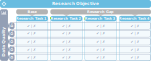
\includegraphics[width=\linewidth]{figures/introduction/objective_dq_grid}
  \caption[Schematic overview of the structural approach taken in this dissertation]{Schematic overview of the structural approach taken in this dissertation. The overall objective of improving scholarly data quality is quantified across data quality dimensions (rows). The approach taken towards this goal is focussed by identifying the research gap and deriving research tasks. Including an initial step of establishing a base upon which the subsequent research is built, four research tasks are identified (columns). The cell contents ``\checkmark | $\times$'' indicate an evaluation of the research task results for the respective data quality dimension.}
  \label{fig:introduction-obj-dq-grid}
\end{figure}

\section{Research Gap and Tasks}\label{sec:intro-gap}

% - volume of data (-> need efficient, robust, fault tolerant processing)
% - multiple modalities (-> need highly generalizable or multiple processing approaches)
% - information sparsity (-> need to bridge gap from visual medium to structured data)
% - specialized content (-> need sophisticated NLP)
% - publishing rate (-> need to frequently update datasets?)
% - ambiguity of labels (-> need ID'ed stuff, need sophisticated NLP)
% - unbounded domain (-> need to cover lots of additional data?)
% - multi-linguality (-> need sophisticated NLP?)

This dissertation is not the first research endeavor with the objective the develop methods for the creation of high-quality scholarly data. Prior approaches exist and, accordingly, have grappled with the challenges laid out in the previous section.
However, there are three key areas of particular importance in which we see shortcomings in existing work. These allow us to focus our efforts of improving scholarly data quality and, as a whole, make up the research gap addressed by this dissertation.
We describe the three areas in the following and, based on that, formulate our research tasks. Figure~\ref{fig:introduction-obj-dq-grid} provides a structural overview of how the research gap and research tasks relate to the previously defined data quality dimensions.

\begin{enumerate}
    \item \textbf{Citation Network} Several of the most prevalent use cases for scholarly data hinge on the interlinking of publications through citations. This includes uses cases such as bibliometric analyses, scientometrics, as well as the study of citation networks as a type of graph (e.g. in graph neural network evaluations). Despite this importance, not much focus seems to be put on the quality of citation networks in scholarly data. The much used data set CiteSeerX~\cite{Wu2015,Wu2016,Patel2021}, for example, takes the approach of clustering references and publications, but there is no assessment of the citation network's completeness---i.e., what proportion of references of a paper can successfully be linked to the cited document. The more recently introduced data set S2ORC~\cite{Lo2020}---more specifically, its \LaTeX\ subset---provides an investigation into the proportion of successfully matched references, but only achieves to successfully match 31.1\% of references.
It stands to reason that data, in which over two thirds of the records are missing a key element, or where the proportion of records missing a key element is unknown, is of insufficient quality.
Improvements regarding citation networks in scholarly data are presented in Chapters~\ref{chp:corpus} and \ref{chp:covgran}. The results presented there entail improvements across all five data quality dimensions.
    \item \textbf{Anglocentrism} Science is a global and therefore inherently multi-lingual endeavor. Accordingly, capturing the state and progress of science in data, necessitates including publications written in various languages. In various areas of NLP, there has been a growing awareness and consideration of non-English language content in the last years~\cite{Dabre2020,Yu2022,Ramesh2023}. However, in research concerned with scientific publications, as well as in available data sets covering scientific publications, there still is a major lack of coverage of non-English documents~\cite{Vera-Baceta2019,Liu2019,Moed2018,Moskaleva2019,MartinMartin2021}.
Accordingly, research results are of limited validity due to an insufficiency of the underlying data.
Improvements regarding the inclusion and analysis of non-English publications are presented in Chapter~\ref{chp:xling}. The presented work entails improvements in the data quality dimensions relevance and comparability.
    \item \textbf{Research Artifacts} To an increasing degree, research is driven by curated data sets and algorithmic processing techniques, such as machine learning methods and models (``research artifacts''). This development can, for example, be observed in the field of NLP, which has undergone a shift towards ``rapid discovery science'', characterized by a high consensus on research topics, methods and technologies~\cite{Jurgens2018}. Further signs of the growing importance of research artifacts are, for example, the launch of both Google Dataset Search\refurl{https://datasetsearch.research.google.com/}{2023-11-24} and Papers With Code\refurl{https://paperswithcode.com/}{2023-11-24} in 2018, as well as the gradual adoption of data citations~\cite{Kratz2015}.
% GDS 2018: https://doi.org/10.1038/d41586-018-06201-x
% PwC 2018: https://web.archive.org/web/20220513185917/https://www.reddit.com/r/MachineLearning/comments/8t0l40/p_papers_with_code_the_latest_machine_learning/
Despite these developments, efforts to include structured representations of research artifacts in scholarly data are limited. Some work in this direction exists, most notably SciERC~\cite{luan2018scierc} and SciREX~\cite{Jain2020scirex}, but it only covers shallow representations of research artifacts.
We argue that shallow representations are insufficient, as they don't provide the necessary granularity for several beneficial applications, such as faceted search and automated reproducibility.
Improvements regarding a more fine-granular coverage of research artifacts are presented in Chapter~\ref{chp:params}. Similar to anglocentrism, the work presented entails improvements in the data quality dimensions relevance and comparability.
\end{enumerate}

In addressing above limitations, we alleviate the state of scholarly data. This improvement is also reflected in the data quality dimensions introduced in Section~\ref{sec:intro-researchobj}, as mentioned for each of the three points above. Details regarding the improvements are tracked along the dissertation, and are summarized at the end of each chapter. The steps to address the identified research gap are structured into four research tasks, described in the following.

\paragraph{Research Tasks}
Based on the research gap identified, we formulate the following four research tasks as sub-points to our overarching research objective set in Section~\ref{sec:intro-researchobj}.

\begin{rtlist}
    \item \textit{Base Methodology} - establish a base methodology for generating a large-scale, high-quality scholarly data set, that is on par with or improving upon existing data sets.
    \item \textit{Citation Network Completeness} - develop a method to link literature references, that is able to link more references than are linked in existing data sets, while not compromising on link correctness or processing efficiency.
    \item \textit{Inclusion of Non-English Publications} - find and implement an approach to include non-English publications into a large-scale, high-quality scholarly data set.
    \item \textit{Fine-gained Research Artifact Representations} - develop a method to extract fine-grained information on research artifacts from text in scientific publications.
\end{rtlist}

% per chapter: cit network, xling, params
% other: cleanliness/precision (but arXMLiv), automation (only compared to ORKG), ...

% others'
% - ORKG
% - OpenAlex(?)
% - Crossref(?)
% - CiteSeer
% - S2ORC

% The Open Research Knowledge Graph (ORKG)~\cite{orkg1,orkg2} provides information on over 28\,k publications, their contributions, research problems addressed etc. For its data, the ORKG is largely reliant on manual or semi-automated data entry.

% CiteSeerX~\cite{Wu2015,Wu2016,Patel2021}, generated from PDF files of various sources, over 10\,M documents, from various fields including medicine and biology, physics, mathematics, and computer science.

% S2ORC~\cite{Lo2020}, generated from PDF files of various sources, over 12\,M documents, from various fields including medicine and biology, physics, mathematics, and computer science.

% limitations
% - 

% USPs of presented work
% - 


%Measuring the Evolution of a Scientific Field through Citation Frames~~\cite{Jurgens2018} (usable here (or in HyperPIE chapter) for extra justification of focus on parameters of used artifacts)

% - - - - - - - - - - - - - - - - - - - - - - - - - - - -

% \begin{infobox-pub}
% \textbf{Publication} \fullcite{Saier2020}
% \end{infobox-pub}

% \begin{infobox-discussion}
% \textbf{Discussion} This text should show what a printed text will look like at this place. If you read this text, you will get no information. Really? Is there no information?
% \end{infobox-discussion}

% \begin{infobox-info}
% \textbf{Remark} This text should show what a printed text will look like at this place. If you read this text, you will get no information. Really? Is there no information?
% \end{infobox-info}

% \begin{infobox-progress}
%       \begin{tabular}{ccl}
%         \toprule
%         Crit.\tnote{a} & Res.\tnote{b} & Explanation \\
%         \midrule
%         \textbf{C1} & {\large\textbf{+}} & Representative coverage in physics, mathematics, CS \\
%         \textbf{C2} & $\circ$ & Primary focus on text content \\
%         \textbf{C3} & {\large\textbf{+}} & $>96$\% accuracy in reference matching \\
%         \textbf{C4} & {\large\textbf{+}} & Low noise due to using \LaTeX\ as data source \\
%         \textbf{C5} & {\large\textbf{+}} & Publications until end of most recent full year \\
%         \textbf{C6} & {\large\textbf{+}} & Provides MAG and arXiv IDs; DOIs in linked MAG \\
%         \textbf{C7} & $\circ$ & Not considered at this stage \\
%         \textbf{C8} & {\large\textbf{+}} & 42.6\% reference matching success rate \\
%         \textbf{C9} & {\large\textbf{+}} & Full-text included \\
%         \bottomrule
%       \end{tabular}
% \end{infobox-progress}

% - - - - - - - - - - - - - - - - - - - - - - - - - - - -

% \section{Research Questions}

% Research questions are provided as a guidance to the reader, giving a high-level perspective on the insights provided by the publications making up this dissertation.

% RQ "formulas":
% Q: "How can <goal> be achieved? A: "<proposed method>"
% Q: "How can <proposed method aspect> be leveraged to achieve <goal>? A: "<proposed method>"
% Q: "What's the nature of <analysis object>?" A: "<analysis result>

\section{Outline and Contributions}

The contributions made across the works tackling the challenges and research gaps outlined above, represent the main part of this dissertation. Together with the following and the final chapter, they make up the remainder of the document, which is structured as follows.

\begin{itemize}
    \item Chapter~\ref{chp:foundations} - \textbf{Foundations}
    \item Chapter~\ref{chp:corpus} - \textbf{Corpus}
    \item Chapter~\ref{chp:covgran} - \textbf{Reference Coverage and Granularity}
    \item Chapter~\ref{chp:xling} - \textbf{References Across Languages}
    \item Chapter~\ref{chp:params} - \textbf{References with Usage Parameters}
    \item Chapter~\ref{chp:conclusion} - \textbf{Conclusion}
\end{itemize}

% The chapters contents are as follows.

In Chapter~\ref{chp:foundations}, Foundations, we introduce overarching and foundational concepts related to scholarly data as well as data mining and information extraction. The provided information is conducive to understanding (1)~decisions made in the system design and method development of the approaches discussed later on, and (2)~the quantification of the research goals and achieved results.

Chapters~\ref{chp:corpus} to \ref{chp:params} make up the main contributions of the work presented in this dissertation. Specifically, these are:

Chapter~\ref{chp:corpus} - \textbf{Corpus}
\begin{itemize}
    \setlength\itemsep{-0.5em}
    \item Contribution: \textit{Linked Document Scholarly Data Corpus Creation from \LaTeX}
    \item Addresses: \rtmark{1}, \rtmark{2}
    \item Improves: relevance, accuracy, timeliness, comparability, and completeness
\end{itemize}
With \emph{unarXive} we present in Chapter~\ref{chp:corpus} a methodology for creating a large-scale corpus of linked, full-text documents from \LaTeX\ source files, which we apply to all of arXiv.org. At the time of publication, it was the first corpus of linked publications with extensive coverage in physics, mathematics, and computer science. By creating the corpus from \LaTeX\ source files, it is less noisy than related work created from PDFs, such as CiteSeerX~\cite{Wu2015}. The creation method furthermore includes a highly accurate reference matching procedure achieving a state-of-the-art matching success rate.
This contribution lays the foundation for the subsequent research conducted for the dissertation, and primarily addresses the research gap \emph{citation network}.
The work presented achieves improvements across all five data quality dimensions.

Chapter~\ref{chp:covgran} - \textbf{Reference Coverage and Granularity}
\begin{itemize}
    \setlength\itemsep{-0.5em}
    \item Contribution: \textit{Inter-Reference Blocking and Fine-Granular Text Representation}
    \item Addresses: \rtmark{2}
    \item Improves: relevance, timeliness, comparability, and completeness
\end{itemize}
Building upon \emph{unarXive}, we present in Chapter~\ref{chp:covgran} advancements in two areas. First, regarding the citation network, we develop a inter-reference blocking and matching method that significantly increases matched references as well as bibliographic couplings, and achieve a new state-of-the-art matching success rate. Second, we present an improved conversion method for \LaTeX\ source files leading to fine-granularly structured document representations. % Consider putting a sentences regarding the updated unarXive here, comparing it to S2ORC (mentioning that S2ORC (LaTeX) pipeline is based on unarXive)
This contribution addresses the research gap \emph{citation network}, and furthermore lays the foundation for the research presented in Chapter 6 (see below).
In total, the work presented achieves data quality improvements in terms of relevance, timeliness, comparability, and completeness.

Chapter~\ref{chp:xling} - \textbf{References Across Languages}
\begin{itemize}
    \setlength\itemsep{-0.5em}
    \item Contribution: \textit{Detection and Large-Scale Analysis of Cross-Lingual Citations}
    \item Addresses: \rtmark{3}
    \item Improves: comparability and completeness
\end{itemize}
Using the \emph{unarXive} corpus, we present in Chapter~\ref{chp:xling} a method to reliably identify cross-lingual citations in English publications. Based on this, we conduct the so far largest analysis of this type of citation. Where previous studies of comparable setting only looked at hundreds of documents, our study includes over one million publications. Analysing cross-lingual citations' prevalence, usage, and impact, we identify trends over time as well as challenges.
This contribution addresses the research gap \emph{anglocentrism}.
The work results in data quality improvements in %the citation network's
terms of 
relevance and comparability.

Chapter~\ref{chp:params} - \textbf{References with Usage Parameters}
\begin{itemize}
    \setlength\itemsep{-0.5em}
    \item Contribution: \textit{Information Extraction for Hyperparameter Information}
    \item Addresses: \rtmark{4}
    \item Improves: comparability and completeness
\end{itemize}
To further improve the granularity of the full-text representations in \emph{unarXive}, we develop in Chapter~\ref{chp:params} information extraction methods for research artifacts and their usage parameters. In doing so, we enable the study of parameter use and reporting patterns across time and scientific disciplines. The extracted information furthermore bears potential for use in automated reproduction. The developed methods achieve an improvement over strong baselines.
This contribution addresses the research gap \emph{research artifacts}.
Regarding data quality, the work represents improvements %regarding the document representation
in the data quality dimensions relevance and comparability.

The dissertation concludes in Chapter~\ref{chp:conclusion}, with an overarching discussion of the results attained, impact of the work so far, and an outlook.

\section{Overview of Publications}\label{sec:intro-puboverview}

The contributions in this dissertation have been published in peer-reviewed international conferences and journals. Table~\ref{tab:primarypublicationoverview} gives an overview of the publications and the chapters they make up. Venue ranks are taken from Core\refurl{http://portal.core.edu.au/conf-ranks/}{2023-10-12} in the case of conferences and from SJR\refurl{https://www.scimagojr.com/}{2023-10-12} in the case of journals.\footnote{The ranks shown are the rating for the respective publication year, or, if not available, the most up-to-date prior ranking. For workshops, the rank of the conference at which the workshop is hosted is shown.} For all publications in Table~\ref{tab:primarypublicationoverview}, the author of this dissertation is the first and corresponding author. Detailed author contributions according to the Contributor Roles Taxonomy\refurl{https://credit.niso.org/}{2023-10-12} are listed at the end of the respective chapter.

\begin{table}[h]
\caption{Overview of publications reused in this dissertation.}
\label{tab:primarypublicationoverview}
  \centering
  % \begin{small}
  \begin{threeparttable}
  \begin{tabular}{crllllr}
    \toprule
    Chapter & Venue & Rank\tnote{a} & Type & Year & Length & Ref. \\
    \midrule
    3 & Scientometrics & SJR Q1 & Journal & 2020 & Full & \cite{Saier2020} \\
    \arrayrulecolor{lightgrey}\cline{1-7}
    \multirow{2}{*}{4} & ULITE@JCDL & Core A* & Workshop & 2022 & Full & \cite{Saier2022ULITE} \\
    \ & JCDL & Core A* & Conference & 2023 & Short & \cite{Saier2023unarXive} \\
    \arrayrulecolor{lightgrey}\cline{1-7}
    \multirow{2}{*}{5} & ICADL & Core A & Conference & 2020 & Full & \cite{Saier2020xling} \\
    \ & IJDL & SJR Q2 & Journal & 2022 & Full & \cite{Saier2021} \\
    \arrayrulecolor{lightgrey}\cline{1-7}\arrayrulecolor{black}
    6 & ECIR & Core A & Conference & 2024 & Full & \cite{Saier2023hyperpie} \\
    \bottomrule
  \end{tabular}
  \begin{tablenotes}
    \item[a] Venue rank in publication year (or closest prior). For workshops, the rank of the hosting conference is shown.
  \end{tablenotes}
  \end{threeparttable}
  % \end{small}
\end{table}

% \begin{table}[h]
% \caption{Overview of publications reused in this dissertation.}
% \label{tab:primarypublicationoverview}
%   \centering
%   \begin{small}
%   \begin{threeparttable}
%   \begin{tabular}{cp{5cm}p{0.7cm}llllr}
%     \toprule
%     Chap. & Publication & Venue & Year & Type & Length & Rank\tnote{a,b} & Ref. \\
%     \midrule
%     3 & unarXive: A Large Scholarly Data Set with Publications’ Full-Text, Annotated In-Text Citations, and Links to Metadata & Scien\-tome\-trics & 2020 & Journal & Full & SJR Q1 & \cite{Saier2020} \\
%     \arrayrulecolor{lightgrey}\cline{1-8}
%     \multirow{2}{*}{4} & A Blocking-Based Approach to Enhance Large-Scale Reference Linking & JCDL & 2022 & Workshop & Full & Core A* & \cite{Saier2022ULITE} \\
%     \ & unarXive 2022: All arXiv Publications Pre-Processed for NLP, Including Structured Full-Text and Citation Network & JCDL & 2023 & Conf. & Short & Core A* & \cite{Saier2023unarXive} \\
%     \arrayrulecolor{lightgrey}\cline{1-8}
%     \multirow{2}{*}{5} & A Large-Scale Analysis of Cross-lingual Citations in English Papers & ICADL & 2020 & Conf. & Full & Core A & \cite{Saier2020xling} \\
%     \ & Cross-Lingual Citations in English Papers: A Large-Scale Analysis of Prevalence, Usage, and Impact & IJDL & 2022 & Journal & Full & SJR Q2 & \cite{Saier2021} \\
%     \arrayrulecolor{lightgrey}\cline{1-8}\arrayrulecolor{black}
%     6 & HyperPIE: Hyperparameter Information Extraction from Scientific Publications & ECIR & 2023 & Conf. & Full & Core A & \cite{Saier2023hyperpie} \\
%     \bottomrule
%   \end{tabular}
%   \begin{tablenotes}
%     \item[a] Venue rank (rating for the publication year, or the most up-to-date ranking if no ranking for publication year is available).
%     \item[b] For workshops, the rank of the conference at which the workshop is hosted is shown.
%   \end{tablenotes}
%   \end{threeparttable}
%   \end{small}
% \end{table}

Additional publications (co-)authored leading up to and during the research period, which are not a direct part of this dissertation but nevertheless informed the overall research trajectory, are listed in Table~\ref{tab:secondarypublicationoverview}.

\begin{table}[h]
  \caption{Overview of secondary publications not reused in this dissertation.}
  \label{tab:secondarypublicationoverview}
  \centering
  % \begin{small}
  \begin{threeparttable}
  \begin{tabular}{rlllclr}
    \hline
    Venue & Rank\tnote{a} & Type      & Year & Length & Pos.\tnote{b} & Ref. \\
    \hline
    BIR@ECIR  & Core A  & Workshop    & 2019 & Full   & 1 of 2 & \cite{Saier2019} \\
    ECIR      & Core A  & Conference  & 2020 & Full   & 1 of 3 & \cite{Saier2020a} \\
    SDP@NAACL & Core A  & Workshop    & 2021 & Short  & 3 of 4 & \cite{Krause2021} \\
    SDU@AAAI  & Core A* & Workshop    & 2022 & Full   & 2 of 3 & \cite{Shapiro2022} \\
    BIR@ECIR  & Core A  & Workshop    & 2022 & Full   & 4 of 5 & \cite{Faerber2022bir} \\
    JCDL      & Core A* & Conference  & 2022 & Full   & 3 of 3 & \cite{Nishioka2022} \\
    JCDL      & Core A* & Conference  & 2023 & Short  & 1 of 3 & \cite{Saier2023cocon} \\
    \hline
    \end{tabular}
    \begin{tablenotes}
      \item[a] Venue rank in publication year (or closest prior). For workshops, the rank of the hosting conference is shown.
      \item[b] Author position.
    \end{tablenotes}
    \end{threeparttable}
    % \end{small}
\end{table}

Especially \cite{Saier2019} and \cite{Saier2020a}, which constitute the results of the master's thesis preceding the doctoral research period, paved the way for this dissertation.
